\documentclass[12pt]{article}
\usepackage{times}
\usepackage{geometry}
\usepackage[english]{babel}
\usepackage[utf8]{inputenc}
\usepackage{fancyhdr}
\usepackage{graphicx}
\usepackage{titlesec}
\usepackage{biblatex}
\usepackage{minted}
\usepackage{xcolor} % to access the named colour LightGray
\definecolor{LightGray}{gray}{0.9}


\addbibresource{References.bib}


\setlength{\headheight}{15.2pt}
\setcounter{secnumdepth}{3}
\rfoot{Pg: \thepage}

\geometry{
   a4paper,
   left = 25mm,
   top = 20mm,
}
\begin{document}
\thispagestyle{empty}

\section*{}
 {\LARGE\makebox[\textwidth]{\textbf{KATHMANDU UNIVERSITY}}}

\centerline{Department of Computer Science and Engineering}
\centerline{Dhulikhel,Kavre}
\begin{figure}[h]
    \centerline{
\includegraphics[width=50.546mm,height=50.546mm]{KU_Logo.png}}
\end{figure}

\centerline{\textbf{A Lab Report}}
\centerline{on}
\centerline{\underline{\textbf{"Lab 1"}}}

\vspace*{12mm}

\centerline{\textbf{[Code No. : COMP 342]}}
\centerline{(For partial fulfillment of 3rd Year/ 1st Semester in Computer Science)}

\vspace*{20mm}

\centerline{\textbf{Submitted by}}
\centerline{\textbf{Aayush Pokharel (Roll No. 43)}}


\vspace*{26mm}


\centerline{\textbf{Submitted to}}
\centerline{\textbf{Dhiraj Shrestha}}
\centerline{\textbf{Dept of Computer Science and Engineering}}

\vspace*{20mm}

\centerline{\textbf{Submission Date: 18th December, 2022}}



\clearpage
\thispagestyle{empty}

\section*{Abstract}
The report is drafted to meet the prerequisites to partially fulfill the COMP 342 course offered by the
Department of Computer Science and Engineering at Kathmandu University. This project is designed
to expand the knowledge of OpenGL,co-ordinate systems and rendering pipeline.
\\\\
\textbf{Keywords:} Co-ordinate systems, OpenGL, rendering

\clearpage
\thispagestyle{empty}
\tableofcontents

\clearpage
\thispagestyle{empty}
\listoffigures

\clearpage
\pagenumbering{arabic}
\section{CHAPTER 1: INTRODUCTION}

\subsection{Environment}
The lab progam was written using the python programming language and OpenGL rendering Library. To write the program a virtual environment is
created and set of libraries is downloaded for the local virtual environment. Then the python interperter runs under this virtual environment
to run the program

\subsection{OpenGL}
The OpenGL rendering library is written in C programming language and a wrapper library called PyOpenGL is available under BSD-style Open-Source licence which translates the
API calls of OpenGL to Python programming.

\subsection{PyGame}
The PyGame is a cross-platform set of Python modules for game development. Despite being a complete package that can handle all the rendering in a highly abstracted manner, the
limitation of only using OpenGL for the lab work required that it only be used as windowing library under a double buffer system and all the relevant rendering process be done by PyOpenGL itself.

\section{CHAPTER 2: CODE}
This is the code for the Lab assignments.
\begin{minted}[
    frame=lines,
    framesep=2mm,
    baselinestretch=1.2,
    bgcolor=LightGray,
    fontsize=\footnotesize,
    linenos
    ]{python}
import pygame as pg
from OpenGL.GL import *
import numpy as np
import ctypes
from OpenGL.GL.shaders import compileProgram, compileShader


class App:
    def __init__(self):

        #initialize python window
        pg.init()
        #getting system's resolution
        width, = pg.display.Info().current_w
        height =  pg.display.Info().current_h
        #printing the resolution to console
        print("Display Width : ", width, "\nDisplay Height : ", height)
        pg.display.set_caption("Lab 1 | Aayush Pokharel")
        pg.display.set_mode((800, 800), pg.OPENGL | pg.DOUBLEBUF)
        self.clock = pg.time.Clock()
        #initialize opengl
        glClearColor(0.1, 0.2, 0.2, 1)
        self.shader = self.createShader(
            "shaders/vertex.txt", "shaders/fragment.txt")
        glUseProgram(self.shader)
        self.flag = Flag()
        self.mainLoop()

    def createShader(self, vertexFilePath, fragmentFilePath):

        with open(vertexFilePath, "r") as f:
            vertex_src = f.readlines()

        with open(fragmentFilePath, "r") as f:
            fragment_src = f.readlines()

        shader = compileProgram(
            compileShader(vertex_src, GL_VERTEX_SHADER),
            compileShader(fragment_src, GL_FRAGMENT_SHADER),
        )

        return shader

    def mainLoop(self):
        running = True
        while running:
            #check events
            for event in pg.event.get():
                if event.type == pg.QUIT:
                    running = False

            #refresh screen
            glClear(GL_COLOR_BUFFER_BIT)

            glUseProgram(self.shader)
            glBindVertexArray(self.flag.vao)
            glDrawArrays(GL_TRIANGLES, 0, self.flag.vertex_count)

            pg.display.flip()

            #timiing
            self.clock.tick(60)

        self.quit()

    def quit(self):

        self.flag.destroy()
        glDeleteProgram(self.shader)
        pg.quit()


class Flag:
    def __init__(self):

        #x,y,z,r,g,b
        self.vertices = (
            -1.0, -1.0, 0.5, 0.0, 0.21, 0.58,
		    0.68, -1.0, 0.5, 0.0, 0.21, 0.58,
		    -1.0, 0.7, 0.5, 0.0, 0.21, 0.58,
								
		    -1.0, 0.0, 0.5, 0.0, 0.21, 0.58,
		    0.72, 0.0, 0.5, 0.0, 0.21, 0.58, 
		    -1.0, 1.0, 0.5, 0.0, 0.21, 0.58,

		    -0.95, -0.95, 0.5, 0.87, 0.04, 0.2,
		    0.55, -0.95, 0.5, 0.87, 0.04, 0.2,
		    -0.95, 0.6, 0.5, 0.87, 0.04, 0.2,
							
		    -0.95, 0.05, 0.5, 0.87, 0.04, 0.2,
		    0.52, 0.05,  0.5, 0.87, 0.04, 0.2, 
		    -0.95, 0.9, 0.5, 0.87, 0.04, 0.2,
            )

        self.vertices = np.array(self.vertices, dtype=np.float32)

        self.vertex_count = 12

        self.vao = glGenVertexArrays(1)
        glBindVertexArray(self.vao)
        self.vbo = glGenBuffers(1)
        glBindBuffer(GL_ARRAY_BUFFER, self.vbo)
        glBufferData(GL_ARRAY_BUFFER,self.vertices.nbytes,
                            self.vertices,GL_STATIC_DRAW)
        glEnableVertexAttribArray(0)
        glVertexAttribPointer(0, 3,GL_FLOAT, GL_FALSE, 24,
                            ctypes.c_void_p(0))
        glEnableVertexAttribArray(1)
        glVertexAttribPointer(1, 3, GL_FLOAT, GL_FALSE, 24, 
                            ctypes.c_void_p(12))

    def destroy(self):
        glDeleteVertexArrays(1, (self.vao,))
        glDeleteBuffers(1, (self.vbo,))


if __name__ == "__main__":
    myApp = App()

\end{minted}

This the code for compiled vertex shader.
\begin{minted}[
    frame=lines,
    framesep=2mm,
    baselinestretch=1.2,
    bgcolor=LightGray,
    fontsize=\footnotesize,
    linenos
    ]{c}
#version 330 core

layout (location=0) in vec3 vertexPos;
layout (location=1) in vec3 vertexColor;

out vec3 fragmentColor;

void main()
{
    gl_Position = vec4(vertexPos, 1.0);
    fragmentColor = vertexColor;
}
\end{minted}
This the code for compiled fragment shader.
\begin{minted}[
    frame=lines,
    framesep=2mm,
    baselinestretch=1.2,
    bgcolor=LightGray,
    fontsize=\footnotesize,
    linenos
    ]{c}
#version 330 core

in vec3 fragmentColor;

out vec4 color;

void main()
{
    color = vec4(fragmentColor, 1.0);

}
\end{minted}
\clearpage
This is the screenshot of the terminal where the virtual environment is set, the relevant packages installed and the program executed.
\begin{figure}[h]
    \centerline{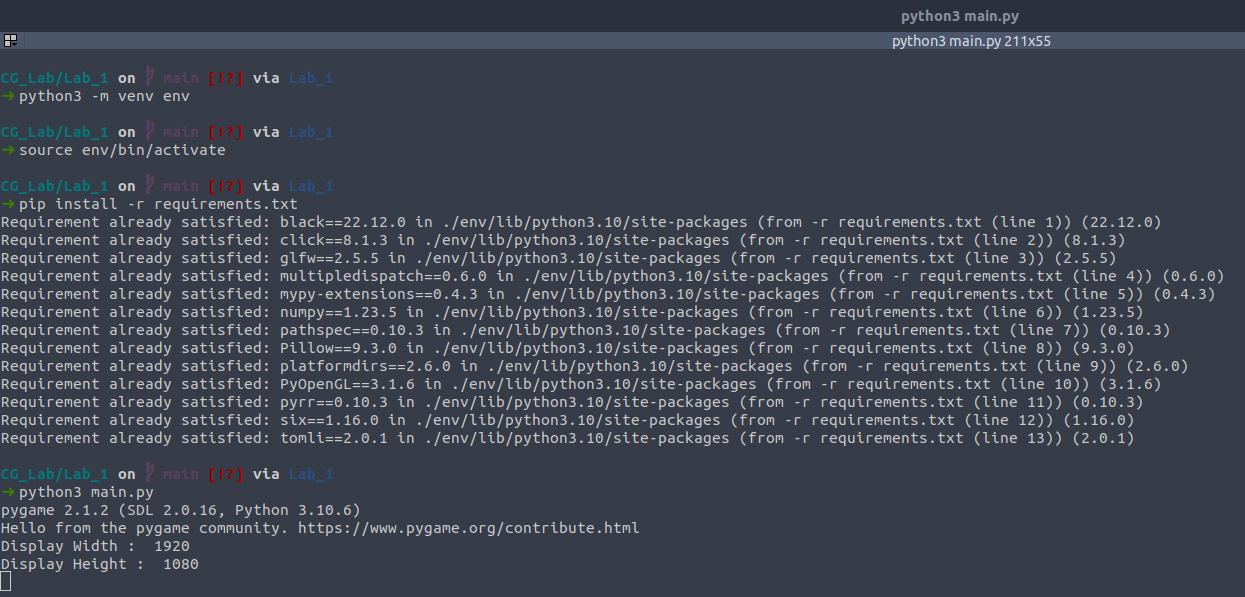
\includegraphics[width=200mm]{Lab1consoletrimmed.png}}
    \caption{Terminal}
    \label{fig}
\end{figure}
\clearpage
This is the screenshot of the executed program.
\begin{figure}[h]
    \centerline{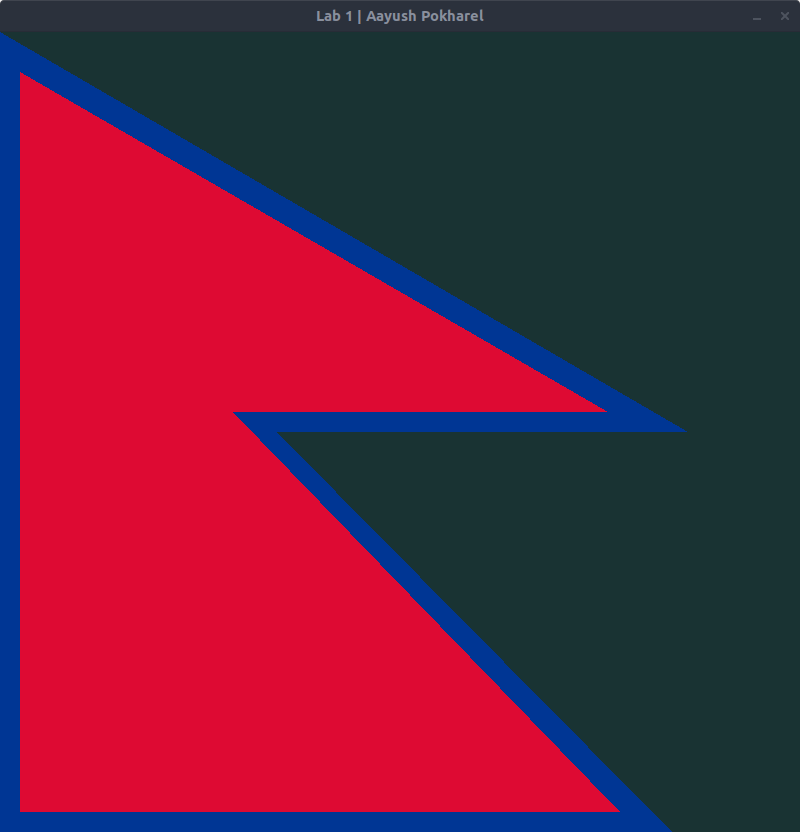
\includegraphics[height=100mm]{flag.png}}
    \caption{App.py}
    \label{fig}
\end{figure}

\section{CHAPTER 3: CONCLUSION}
In the nutshell, the lab was was short and consisted of pretty easy tasks that could help a user to
familirize oneself with the rendering pipeline but it was very time consumming to learn the OpenGL rendering pipline
and the lack of instructions on which pipeline and methodlogy to follow (old methodlogy or programmable shader) led to some
confusion and being faced with unknown-unknown elements from the redering pipeline and library while intially writing the program.
\clearpage
\thispagestyle{empty}
\printbibliography

\end{document}